
\begin{figure}[h!]
    \centering
    \caption{Estimates of the effect of the minimum wage on rents, baseline sample
             including leads and lags}
    \label{fig:dynamic_workplace}

    \begin{subfigure}{.65\textwidth}
        \caption{Estimates in first differences}
        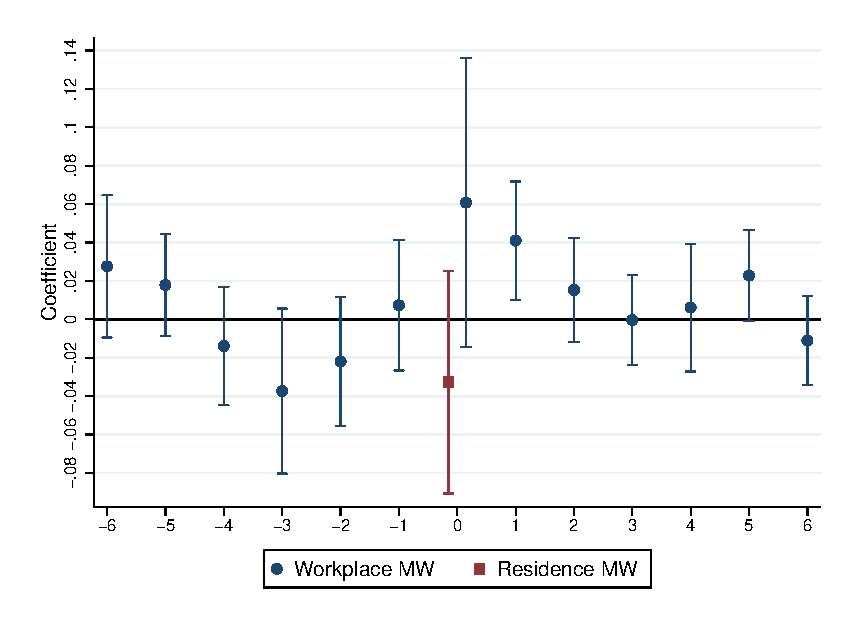
\includegraphics[width = 1\textwidth]
            {fd_baseline/output/fd_both_mw_wkp_only_dynamic}
    \end{subfigure}\\
    \begin{subfigure}{.65\textwidth}
        \caption{Implied path in levels}
        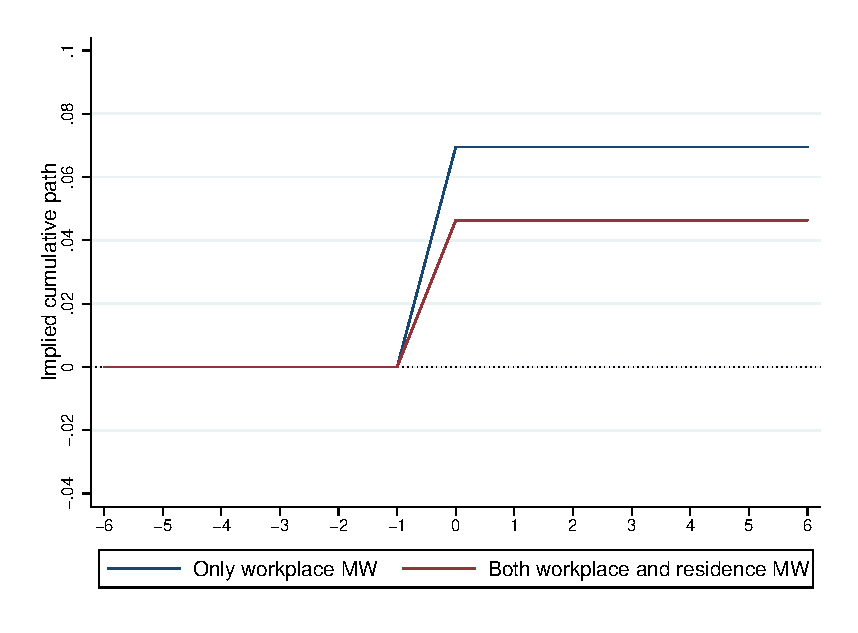
\includegraphics[width = 1\textwidth]
            {fd_baseline/output/implied_cumulative}
    \end{subfigure}

    \begin{minipage}{.95\textwidth} \footnotesize
        \vspace{3mm}
        Notes:
        Data are from the baseline estimation sample described in Section 
        \ref{sec:data_final_panel}.
        The top panel shows coefficients from regressions of the change in 
        log of rents per square foot on leads and lags of the change in the 
        workplace MW and the change in the residence MW.
        The bottom panel shows the implied paths in levels given the estimated 
        coefficients.
        The regression includes time-period fixed effects and economic controls 
        that vary at the county by month and county by quarter levels.
        The measure of rents per square foot correspond to the Single Family, 
        Condominium and Cooperative houses from Zillow.
        The residence MW is defined as the log statutory MW in the same ZIP code.
        The workplace MW is defined as the log statutory MW where the average 
        resident of the ZIP code works, constructed using LODES 
        origin-destination data.
        Economic controls from the QCEW include the change of the following 
        variables: the log of the average wage, the log of employment, and 
        the log of the establishment count for the sectors 
        ``Information,'' ``Financial activities,'' and ``Professional and 
        business services.''
        95\% pointwise confidence intervals are obtained from standard errors 
        clustered at the state level.
    \end{minipage}
\end{figure}
